\begin{frame}
\frametitle{Latest (good) news on AI in radiology}
\small
\begin{columns}[T]
    \begin{column}[T]{0.5\textwidth}
    \begin{center}
       \vspace{-5mm}
        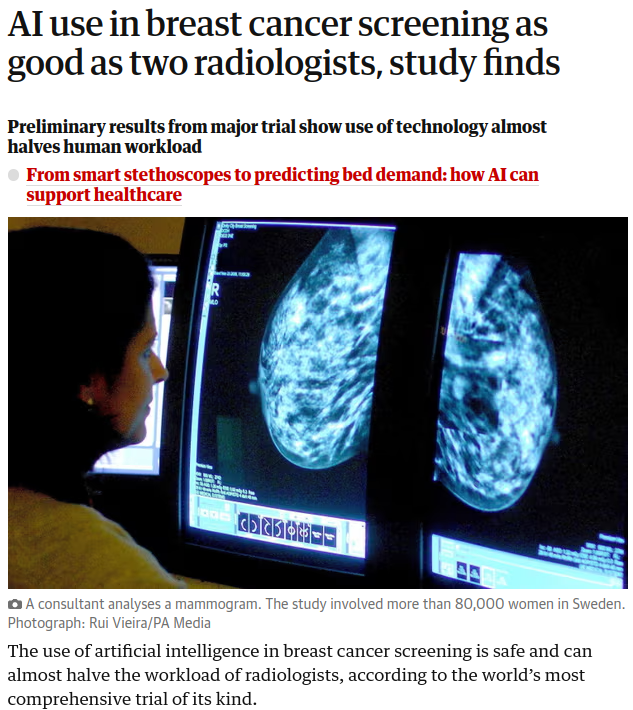
\includegraphics[width=0.9\textwidth]{./misc_images/radiology_1}
        
    \end{center}
    \footnotesize{This is a machine learning classification example: Classification is based on similarity to labeled training images.}
        
    \end{column}


    \begin{column}{0.49\textwidth}
    
    Note the implementation:
    \begin{itemize}
    \item AI is combined with humans 
    \item AI pre-screens before human
    \item Previous studies have indicated that AI can have better sensitivity but lower specificity then humans
    \end{itemize}

    Questions....
    \begin{itemize}
    \item How transferable will the method be (different imagers, different patient populations)?
    \item Is accuracy compared to humans the best measure?
    \end{itemize}
    \end{column}
\end{columns}

\end{frame}